\documentclass[aps,prb,reprint]{revtex4-1}
\usepackage{graphicx}
\usepackage{bm}
\makeatletter

\begin{document}

\title{Statement of Interest: A horizon of science to be cultivated by X-ray engineering}
\author{Nobuyoshi Hiramatsu}

\maketitle

%Motivation Ph.D.
Photonics and physics of measurement\cite{Ozawa} have been my general interests over the past few years. From this point of view, my research experiences including magneto-spectroscopy at Kono lab in Rice university (Nakatani RIES program Part I), a research project of mid-infrared plasmonics in my home university, and 5-month-intern developing optical smoke detectors at a semiconductor-sensor manufacturer were motivated. Through the experiences communicating with highly specialized researchers, I realized the necessity to grow up my strength to be a core competence in a specific discipline by pursuing Ph.D. $\:$In that sense, a spectroscopic experiment utilizing a special magnetic system at Kono group, which system is one of their strengths, has been especially enlightening to make me consider my prospective competences. Among my extensive interests over light and measurement, I believe particularly x-ray physics as probe of nature to be worth concentrating in for possible Ph.D. degree, because of its promising development, importance for frontier science, and an increasing demand of x-ray engineers as described below.

%Promising development
Figure 1 shows rapid enhancement in functionality of x-ray sources for the last several decades\cite{Als-Nielsen}, by characterizing a quality of emitted x-ray. By considering general history of optical physics in various wavelength regime that inventions of light sources have led further development and applications of the field, I would also expect relatively unexplored x-ray physics follows the source development. Compact and efficient new-generation sources have been intensively studied to diffuse x-ray sources for laboratory use and the sake of x-ray physics as a whole, based on laser-driven plasma-wave electron accelerators\cite{Hooker}, inverse Compton scattering\cite{Fukuda}, and high-order harmonic generation by mid-infrared pulse\cite{Popmintchev,Weisshaupt}.  
From my standpoint, experiences with these convenient sources are quite attractive for my near future, since they should replace the current large facilities to become dominant sources.

%Training
Reflecting development of the technologies, trained x-ray engineers supposed to be in increasing demand for the next few decades. Inherent harm aspect of x-ray for human health\cite{Gonzalez} and special x-ray optics support their importance. In other words, a well-trained skill set with x-ray engineering can be my future strength of research career. Therefore, practical training in x-ray engineering will be highly beneficial to familiarize myself in x-ray engineering, and I am determined to apply for the great opportunity based on the Nakatani RIES program Part II.

%LBNA
As described above, I am interested in practical training with compact x-ray sources. In particular, it would be grateful if I could work with Dr. Cameron Geddes who is a leading specialist of the compact sources at Berkeley Lab Laser Accelerator Center in Lewrence Berkeley National Laboratory (LBNA). I am also interested in discussion with researchers in LBNA and Stanford Linear Accelerator Center, where historically played an important role as the hub of x-ray associated projects, and still leading the world.

%Beyond x-ray
I lastly note future work of experimental physics beyond x-ray regime.
Above photon energy of $\sim \mathrm{1\:TeV}$ (electron-weak scale) by multiple orders higher than x-ray photon energy, photons are no longer distinguishable from other elementary particles owing to revival of electroweak symmetry\cite{Barklow}. In a word, light may behave in a different way.
I dream, x-ray engineering dealing with high-energy photonics helps experimental research of such a energetic particle, heralding new science.
%Why do you want to participate in the Part II program? How will this experience further your long-term goals and build upon your prior experience in the Part I program? What type of research are you most interested in pursuing during the Part II program? Do you have any potential host professors and universities that you are interested in for the Part II program?

\setlength\textfloatsep{0.8em}
\setlength\abovecaptionskip{0em}
\begin{figure}[b]
  \center
    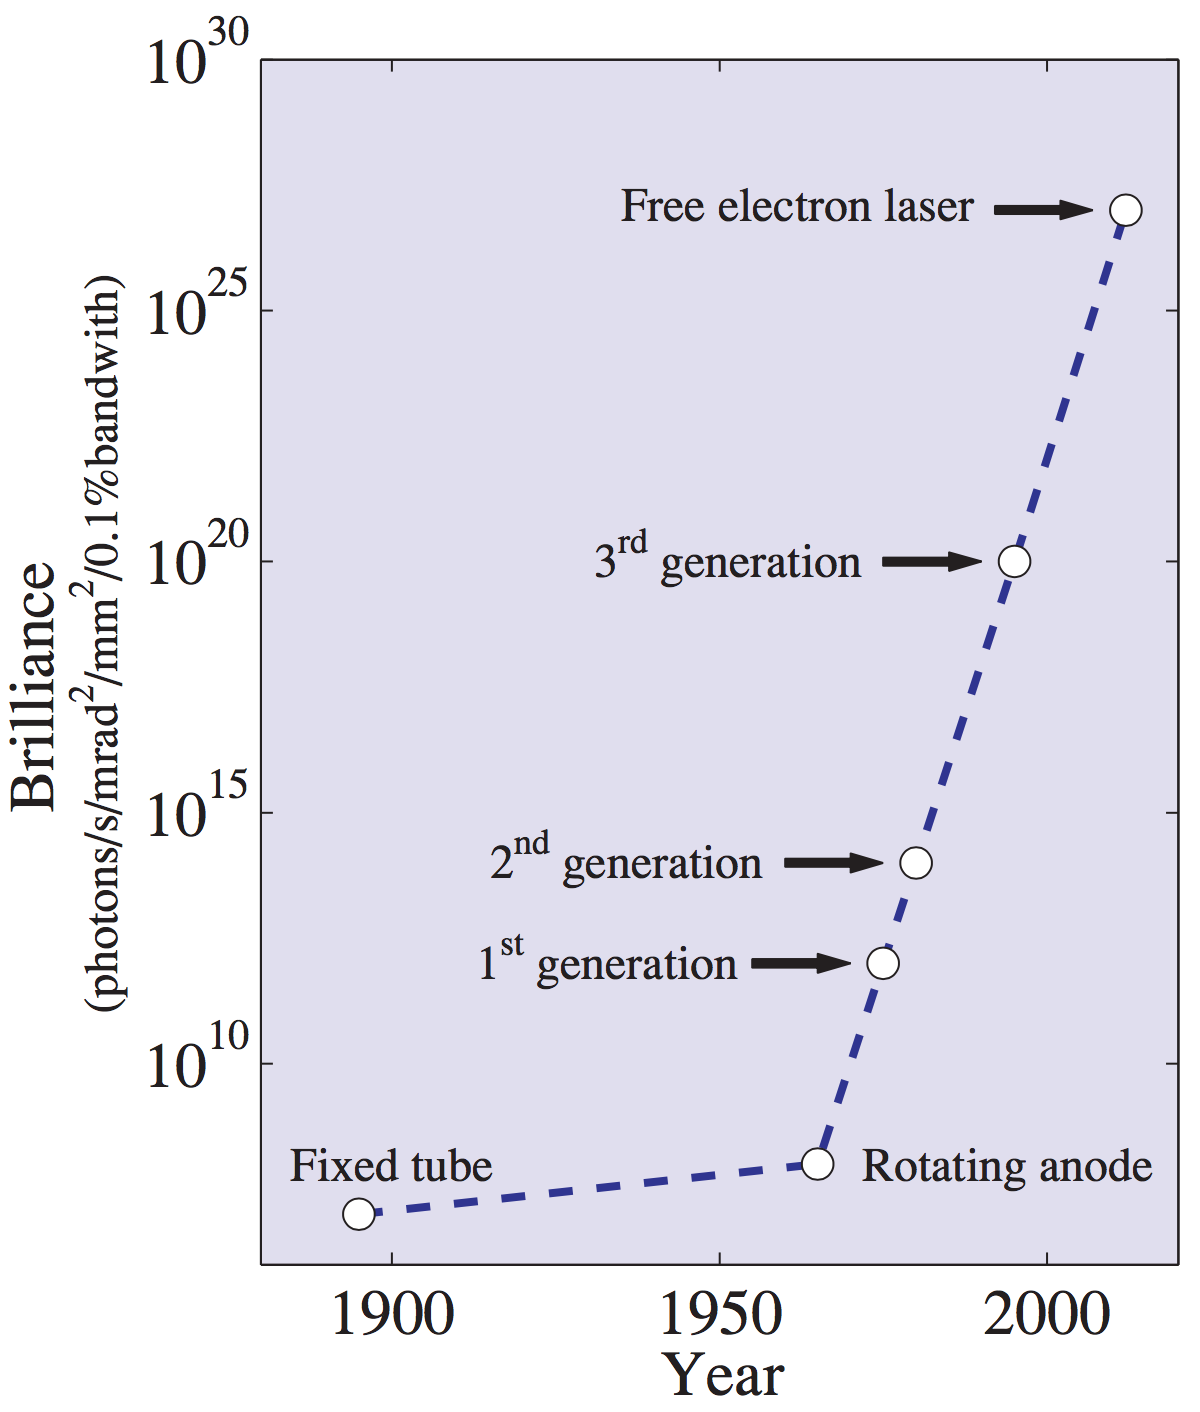
\includegraphics[width=0.6\hsize]{Brilliance.eps}
     \label{fig:brilliance}
     \caption{Development of x-ray sources.}
\end{figure}

%\vspace{-1em}
%\renewcommand{\refname}{}
\bibliography{Statement_of_interest_bib}

\end{document}